\begin{figure*}
        \centering
        \begin{subfigure}[b]{0.475\textwidth}
            \centering
            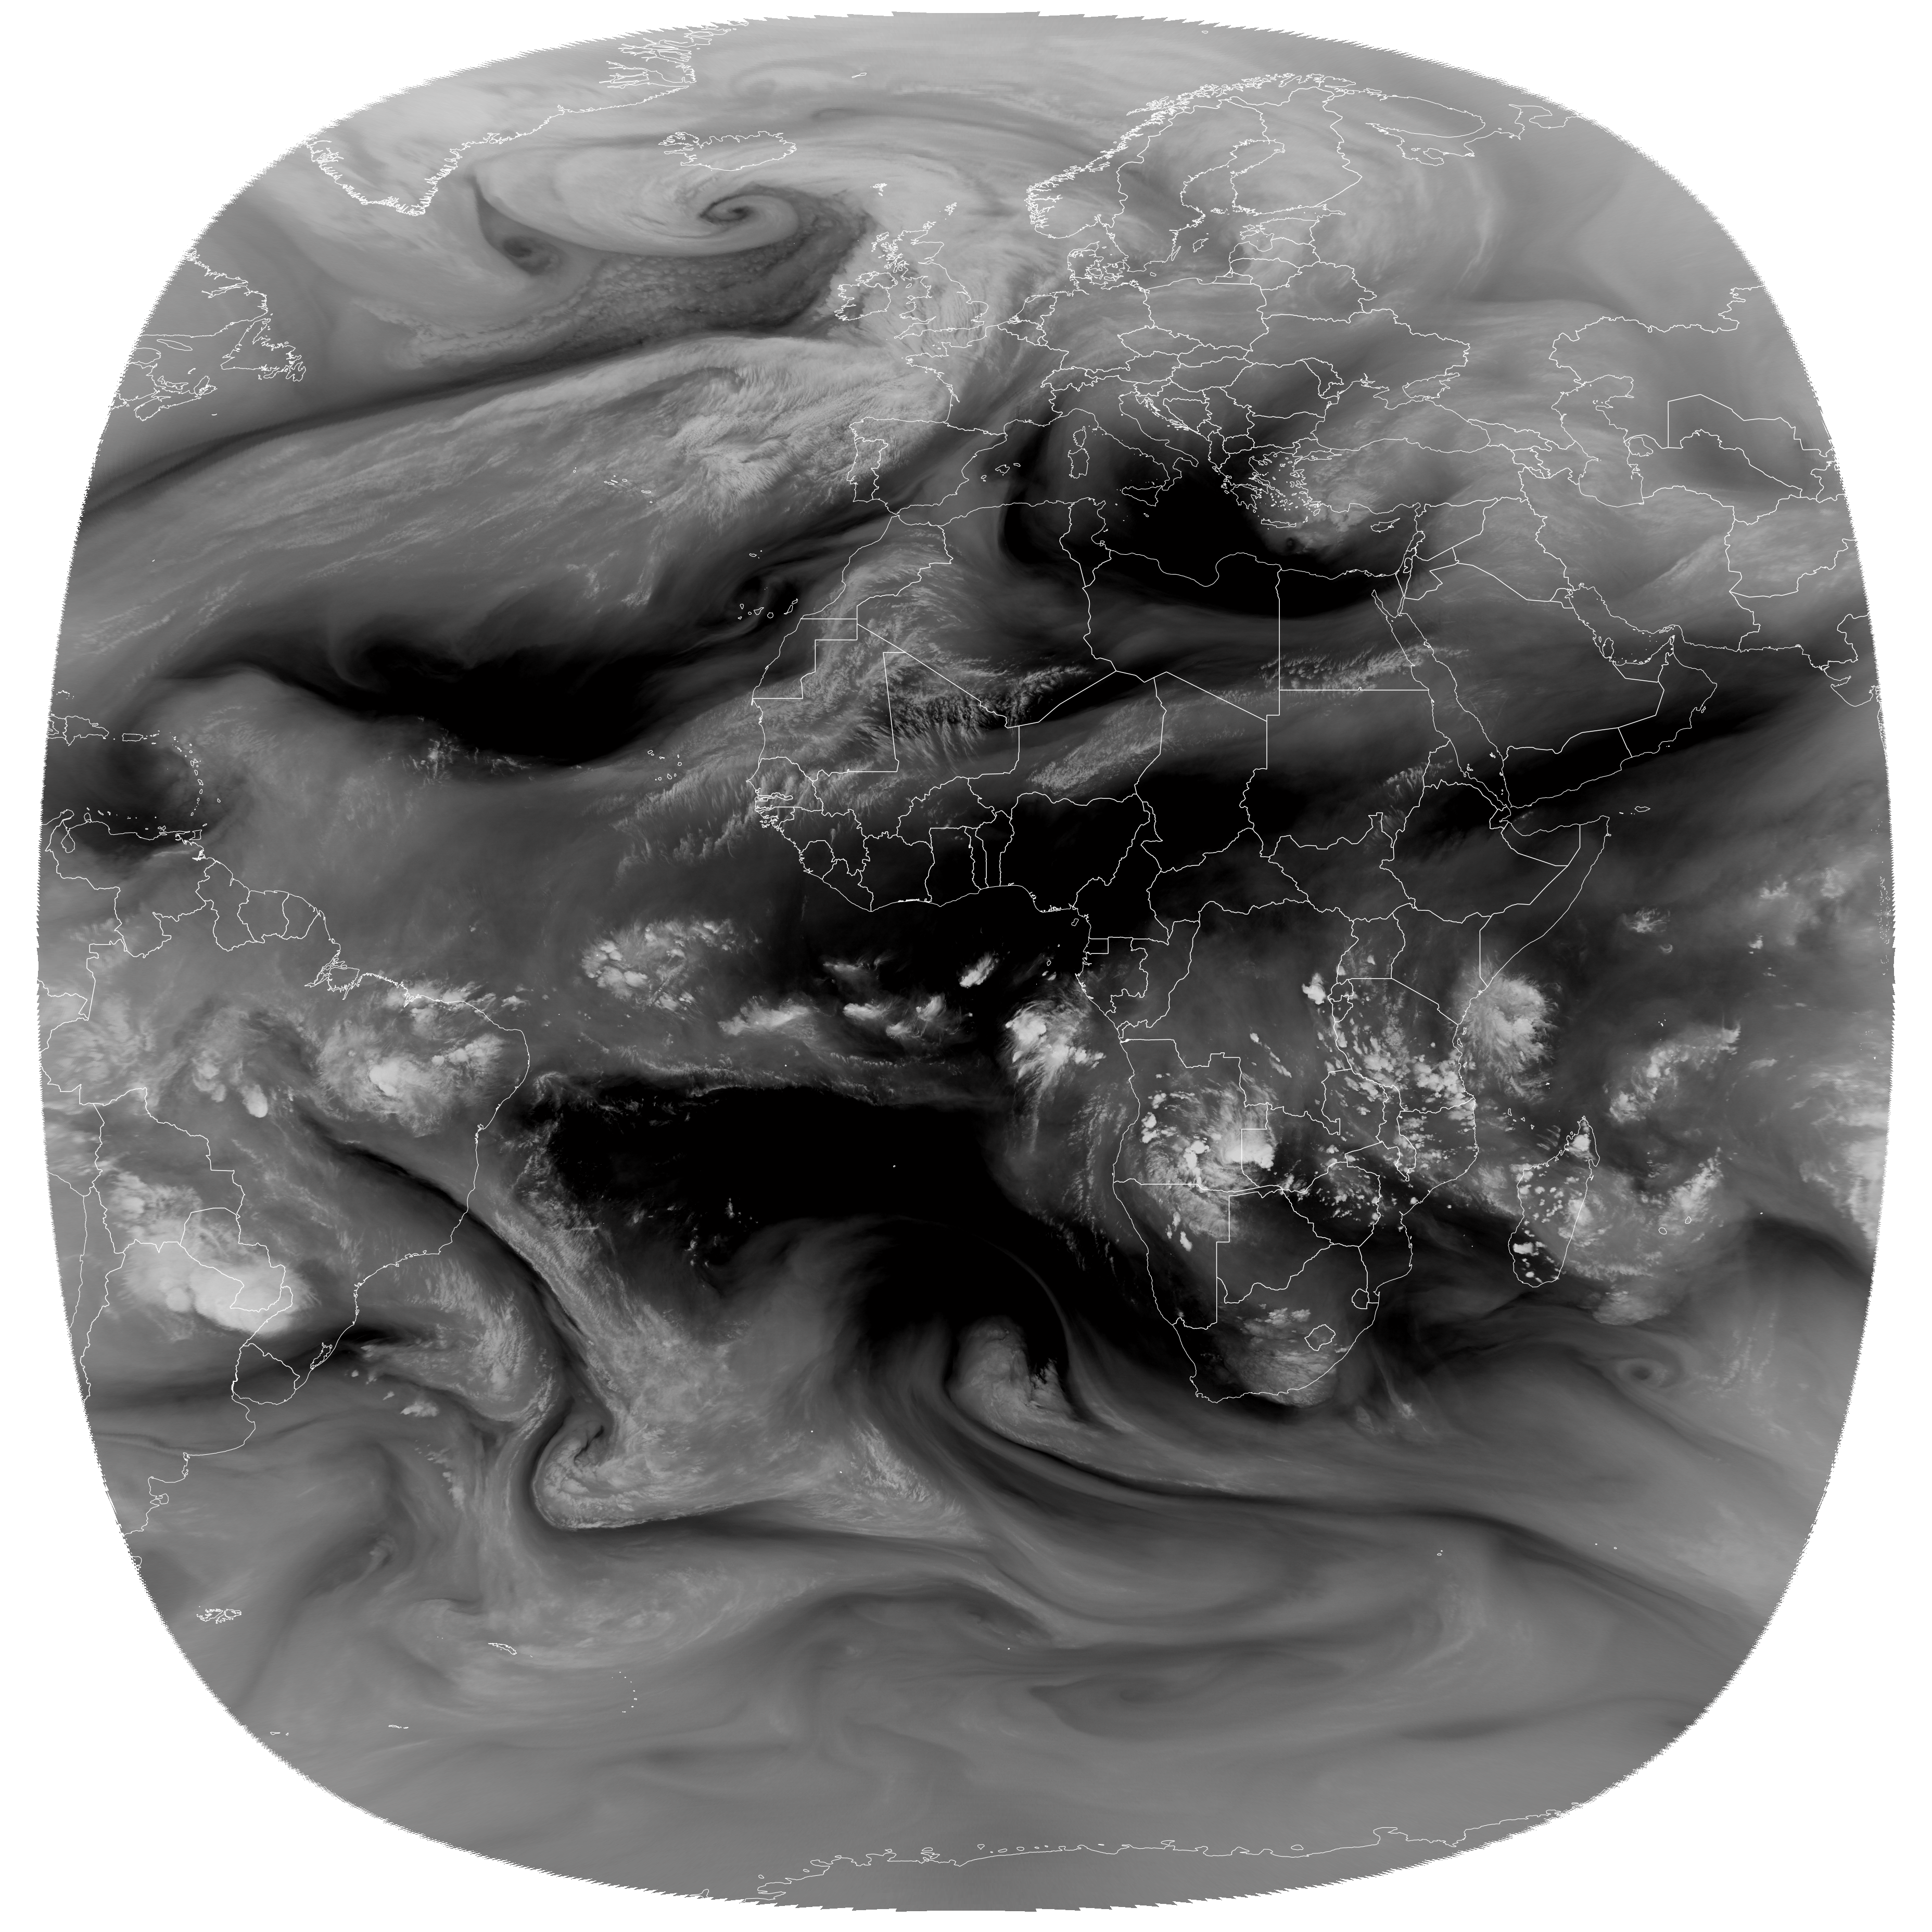
\includegraphics[width=\textwidth]{Chapter2_Theory/images/sat_channels/meteosat-msg_wv062_overlay-ne_10m_coastline_overlay-ne_10m_admin_0_boundary_lines_land.png}
            \caption[Channel WV 6.2]%
            {{\small Channel WV 6.2}}    
            \label{fig:WV_6.2}
        \end{subfigure}
        \hfill
        \begin{subfigure}[b]{0.475\textwidth}  
            \centering 
            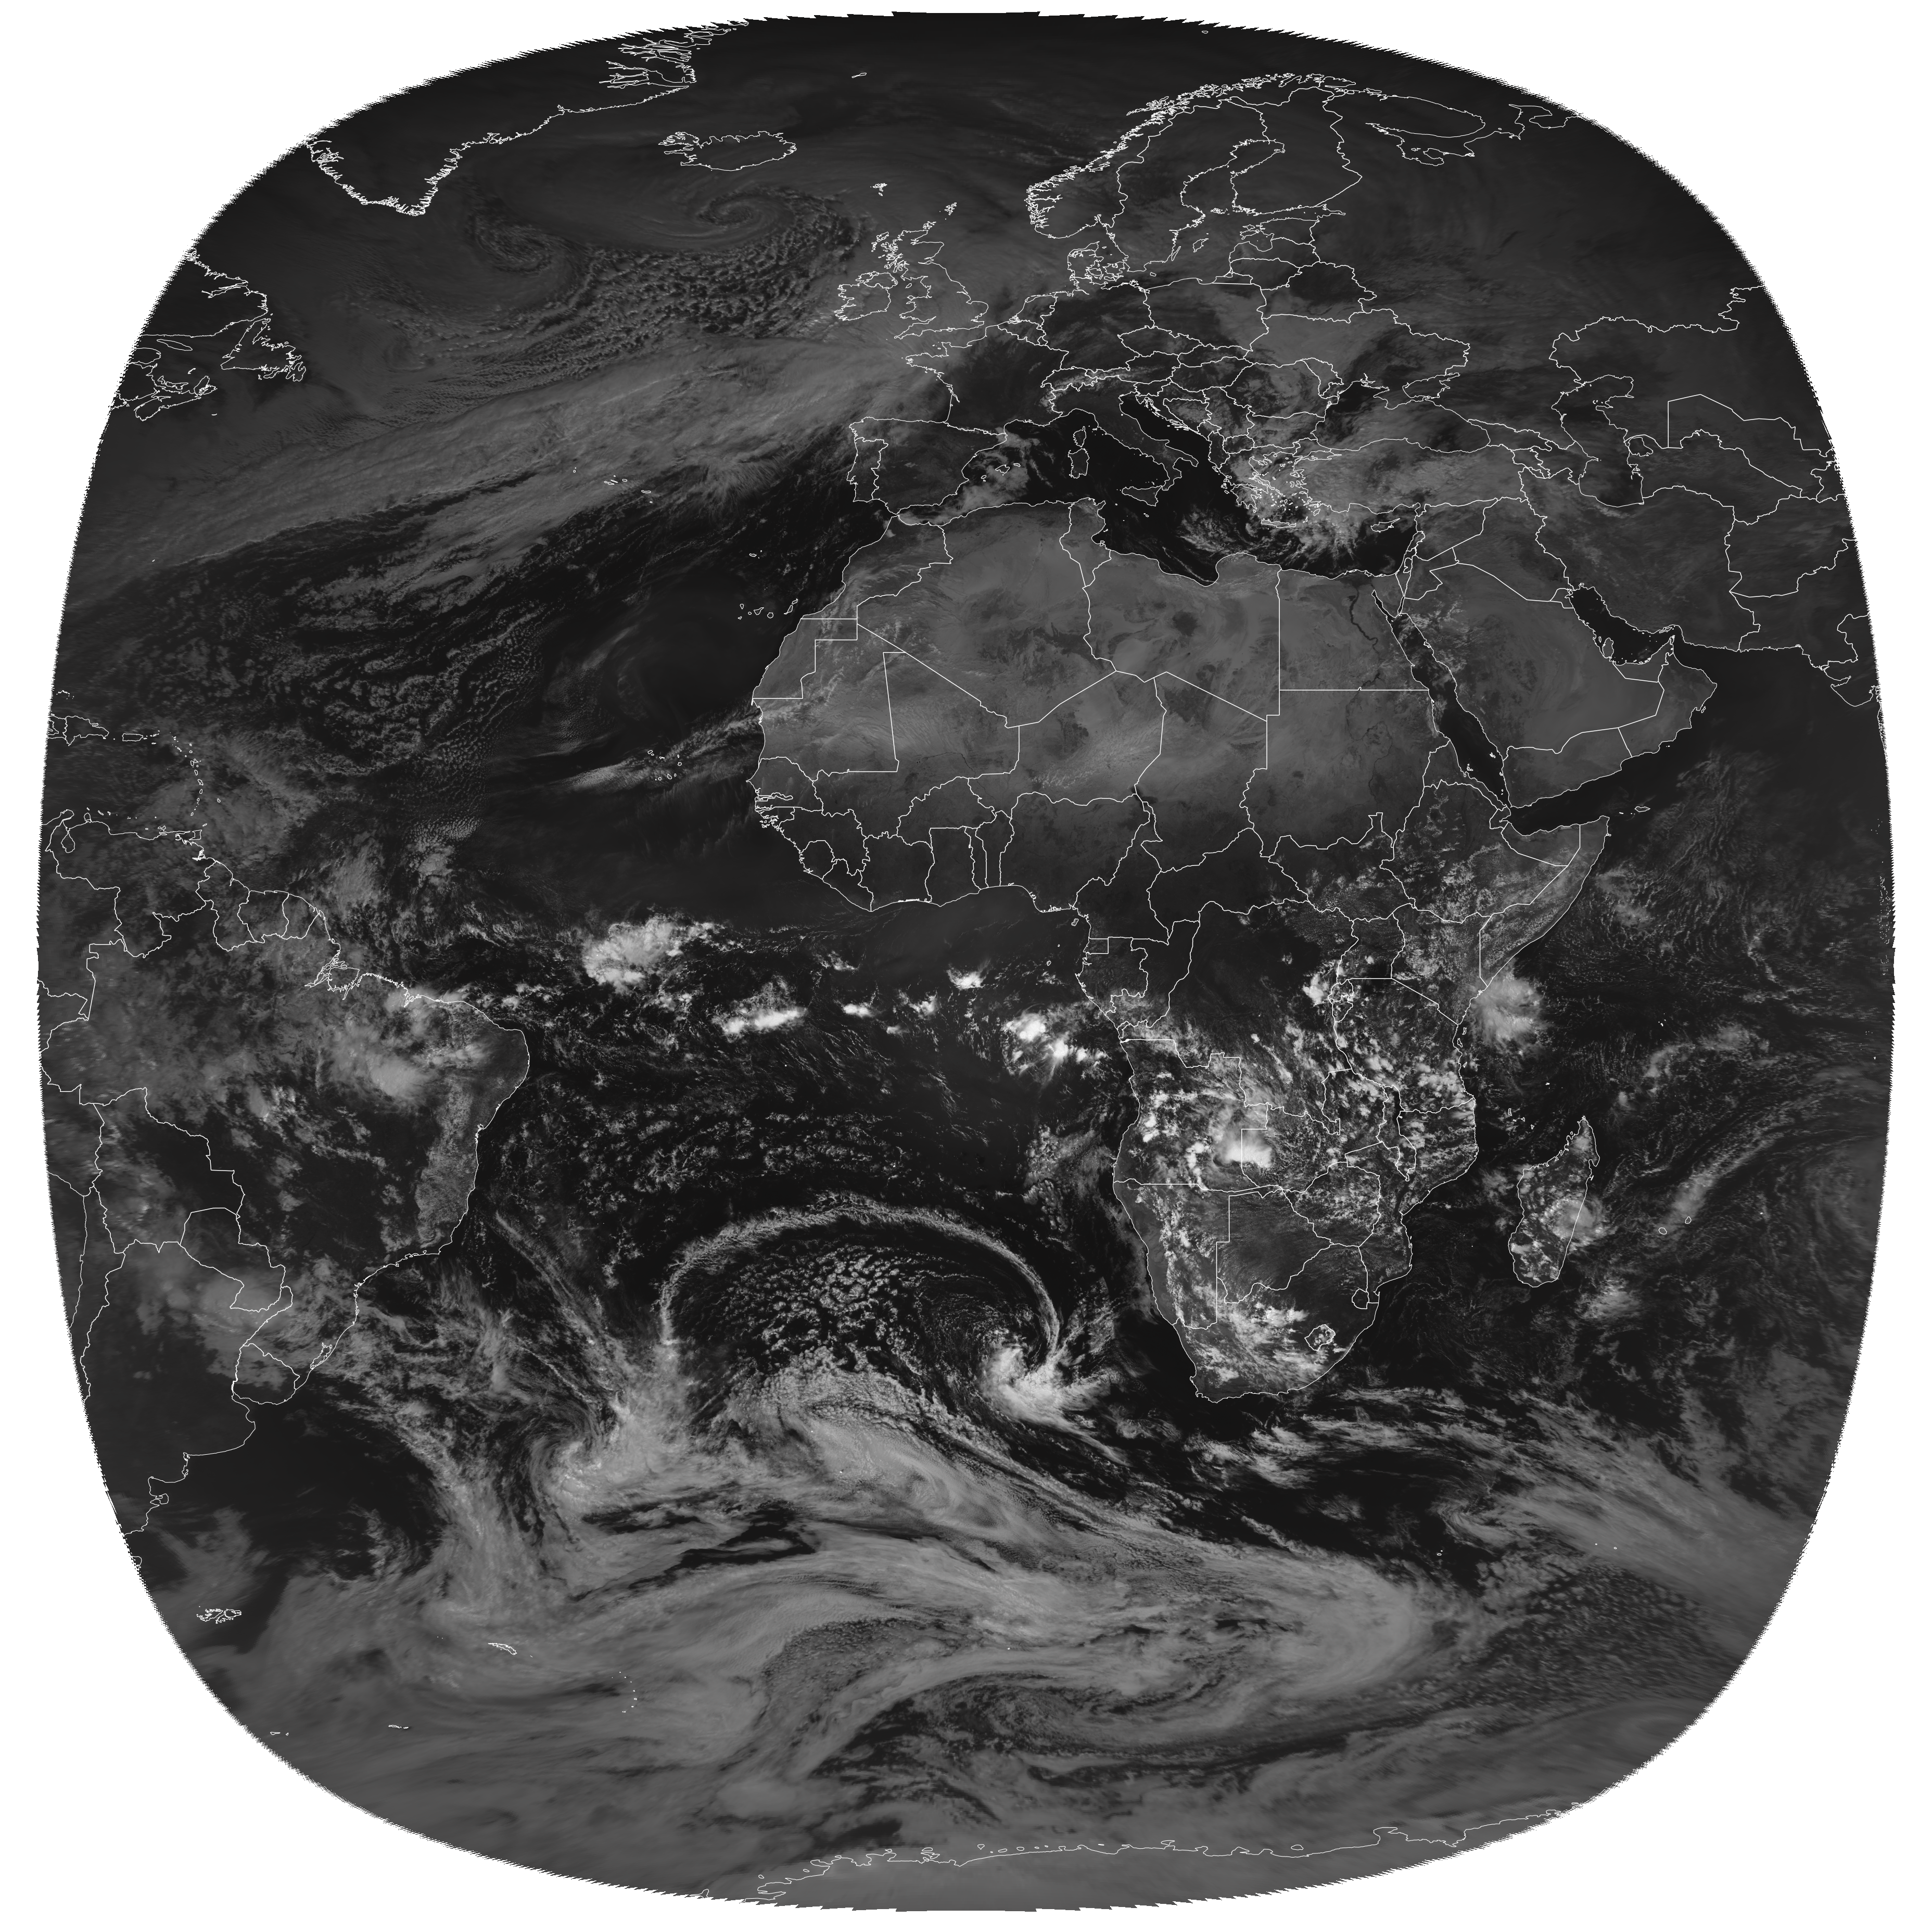
\includegraphics[width=\textwidth]{Chapter2_Theory/images/sat_channels/meteosat-msg_vis006_overlay-ne_10m_coastline_overlay-ne_10m_admin_0_boundary_lines_land.png}
            \caption[]%
            {{\small VIS 0.6}}    
            \label{fig:VIS_0.6}
        \end{subfigure}
        \vskip\baselineskip
        \begin{subfigure}[b]{0.475\textwidth}   
            \centering 
            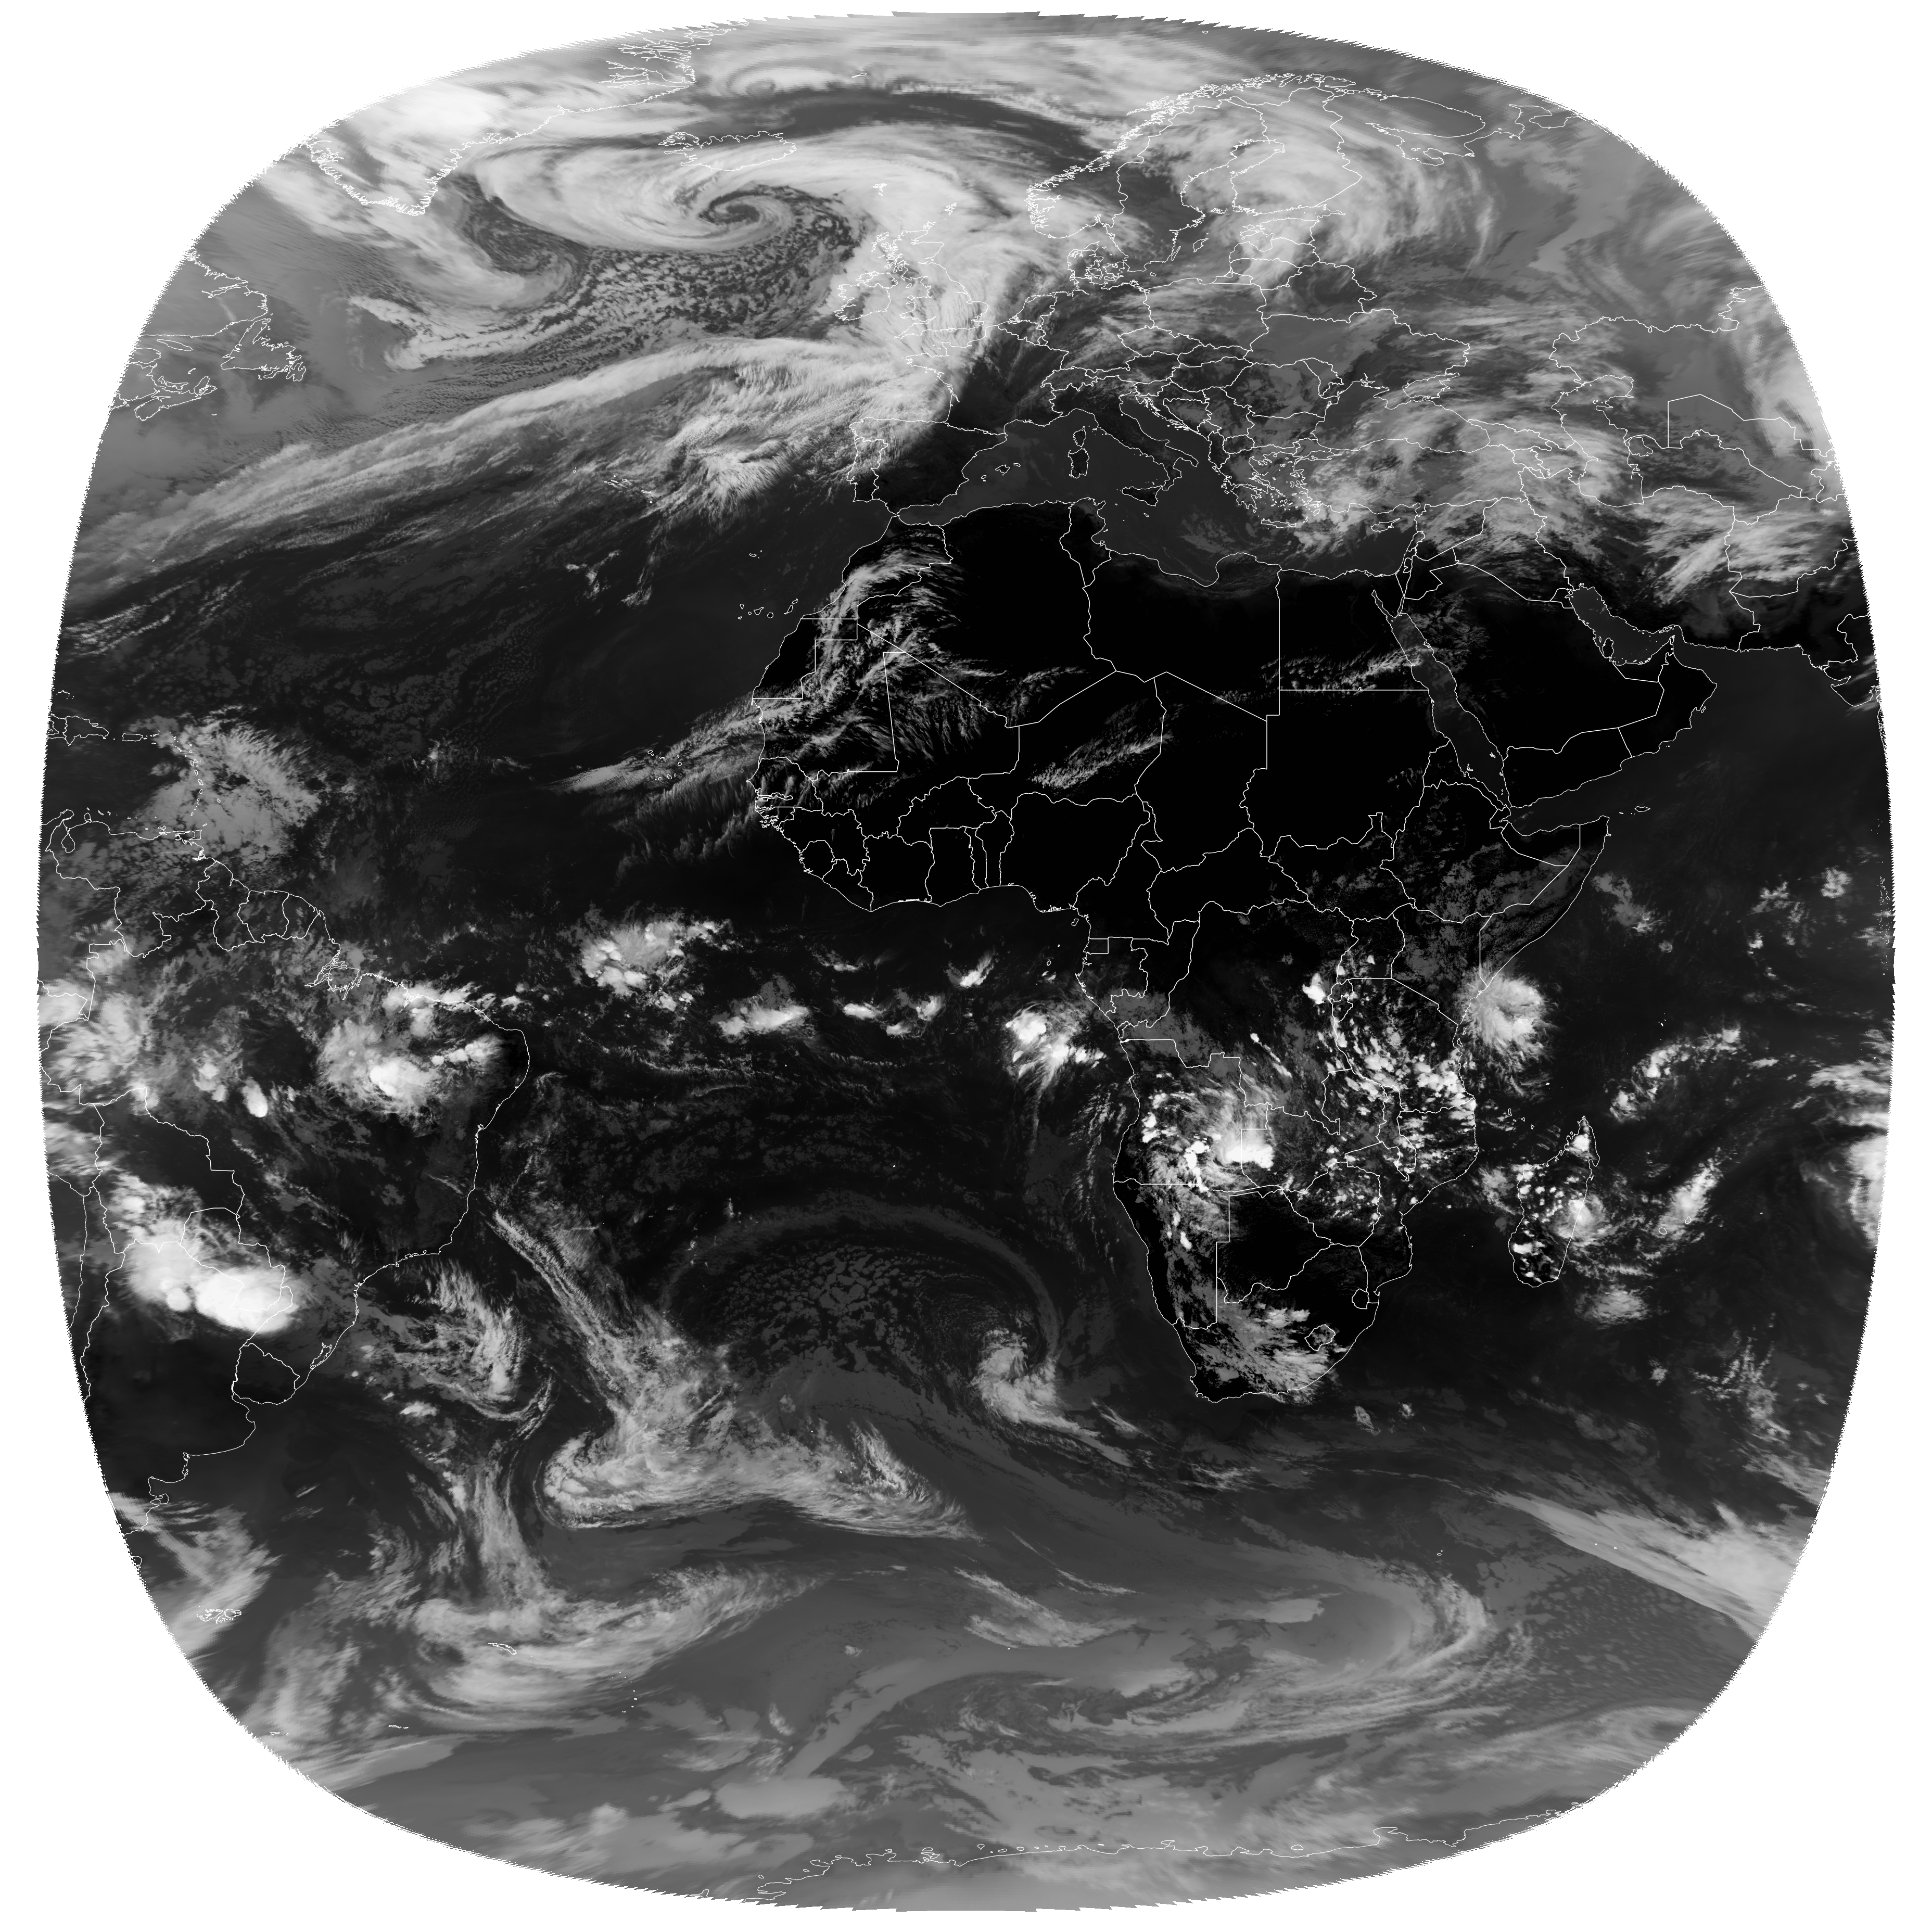
\includegraphics[width=\textwidth]{Chapter2_Theory/images/sat_channels/meteosat-msg_ir108_overlay-ne_10m_coastline_overlay-ne_10m_admin_0_boundary_lines_land.png}
            \caption[something]%
            {{\small IR 10.8}}    
            \label{fig:IR_10.8}
        \end{subfigure}
        \quad
        \begin{subfigure}[b]{0.475\textwidth}   
            \centering 
            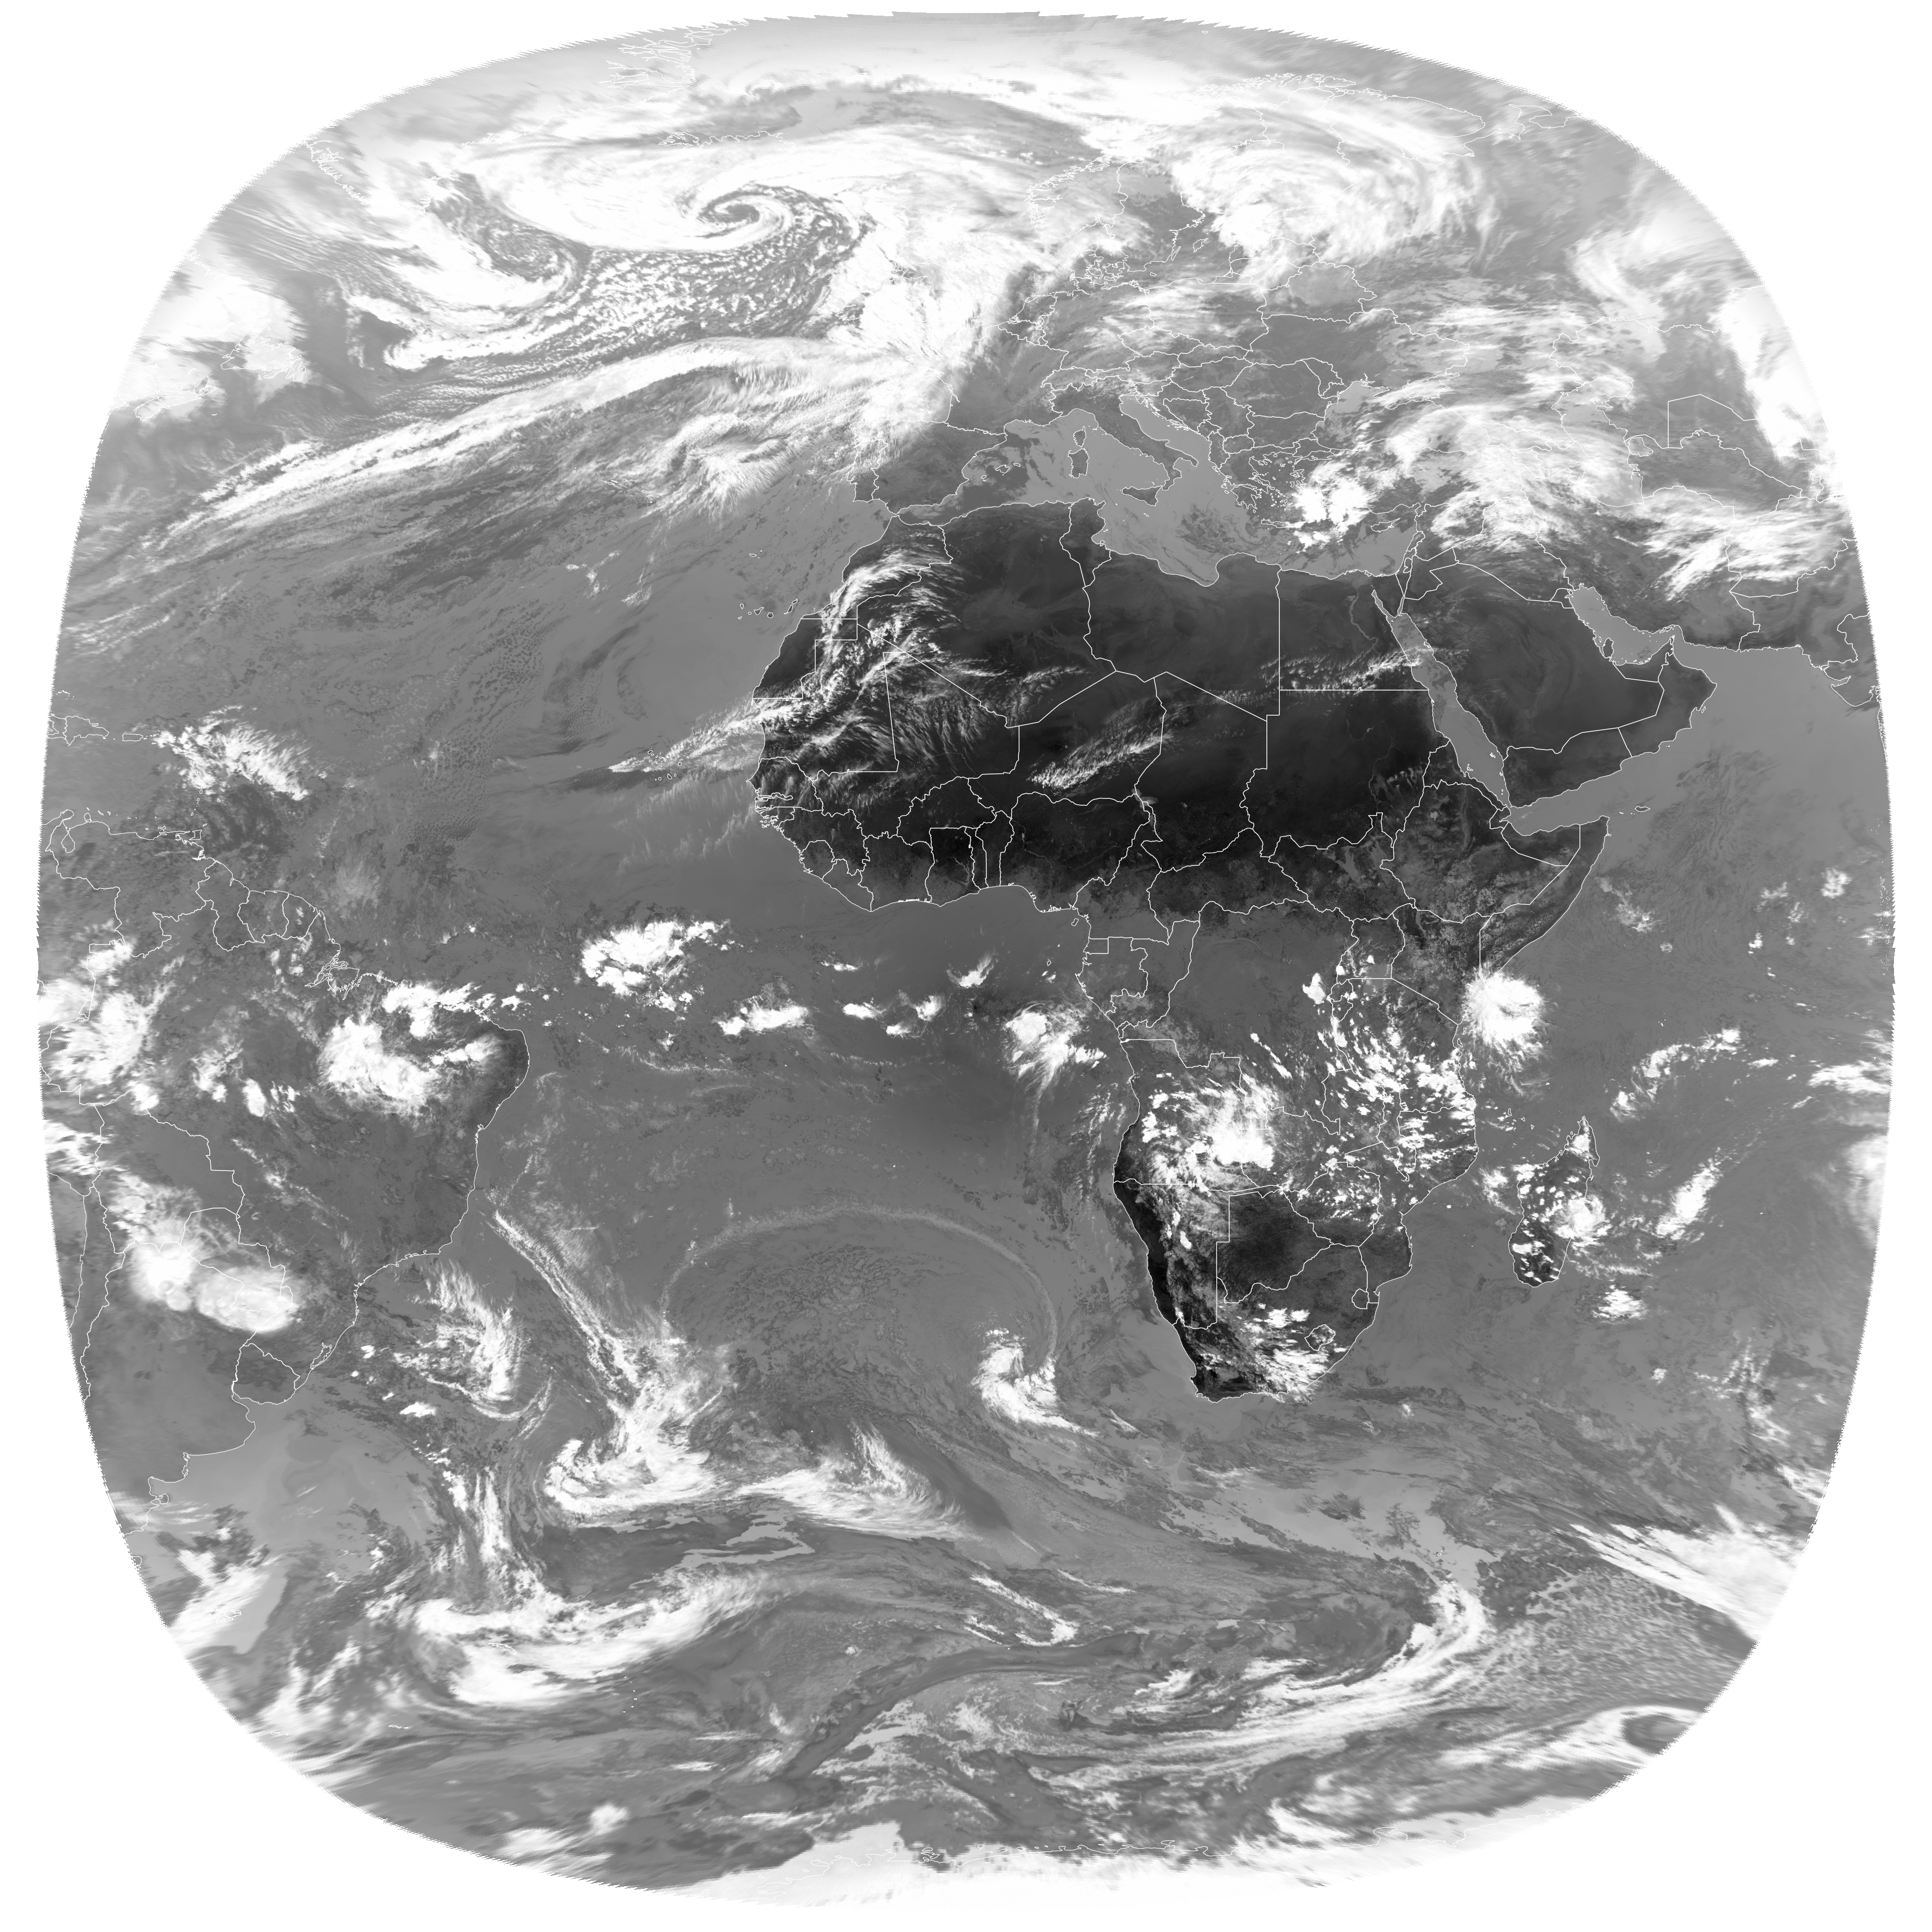
\includegraphics[width=\textwidth]{Chapter2_Theory/images/sat_channels/meteosat-msg_ir039_overlay-ne_10m_coastline_overlay-ne_10m_admin_0_boundary_lines_land.png}
            \caption{{\small IR 3.9}}    
            \label{fig:IR_3.9}
        \end{subfigure}
        \caption{{Spectral bands from SEVIRI. February 15th 2020 at noon. It shows the lowpressure system \textit{Elsa} positioned of the west coast of Iceland. Having a record breaking low of 915hPa (\cite{nrk_lavtrykk}). 
        The images are provided by  \cite{eumetcast_image_gallery}.}
    } 
    \label{fig:SEVIRI_channels}
\end{figure*}

% Info på bildene \textbf{Rectified (level 1.5) Meteosat SEVIRI image data. The data is transmitted as High Rate transmissions in 12 spectral channels. Level 1.5 image data corresponds to the geolocated and radiometrically pre-processed image data, ready for further processing, e.g. the extraction of meteorological products. Any spacecraft specific effects have been removed, and in particular, linearisation and equalisation of the image radiometry has been performed for all SEVIRI channels. The on-board blackbody data has been processed. Both radiometric and geometric quality control information is included. Images are made available with different timeliness according to their latency: quarter-hourly images if latency is more than 3 hours and hourly images if latency is less than 3 hours (for a total of 87 images per day). To enhance the perception for areas which are on the night side of the Earth a different mapping with increased contrast is applied for IR3.9 product. The greyscale mapping is based on the EBBT which allows to map the ranges 200 K to 300 K for the night and 250 K to 330 K for the day.}
% Lastet ned 16.02.2020.